\chapter{Bearings Faults Diagnostics and Prognostics}%
\label{chapter:bearings_faults_diagnostics_and_prognostics}

\chapterintrobox{Vibration condition monitoring are vital for many industrial systems, vibration data contains very useful information about health state of the equipment and the fault type. Nevertheless, gaining insights from vibration signals in real-world applications turns out to be a complex—and in many times, unfruitful—process. This is mainly due to the complexity of the problem. This chapter introduces several approaches where neural networks are used for diagnostics and prognostics of bearings elements}

\section{Case Western Reserve University Bearings Data}

\begin{wrapfigure}{r}{0.5\textwidth}
    \centering
	\begin{tikzpicture}
	\node (outer) at (3.5,1.2) {\makecell{\small Outer\\Race}};
	\node (inner) at (3.5,0) {\makecell{\small Inner\\Race}};
	\node (ball) at (3.5,-1.2) {\makecell{\small Ball\\(in cage)}};
	
	\node (outer2) at (1.3,1.2) {};
	\node (inner2) at (.3,0) {};
	\node (ball2) at (-.5,-1.2) {};

	\node[inner sep=0] (image) at (0,0) {\includegraphics[width=0.35\textwidth]{figures/skf.jpg}};

	\draw [|->,  thick, red] (outer.west) -- (outer2);
	\draw [|->,  thick, red] (ball) -- (ball2);
	\draw [|->,  thick, red] (inner) -- (inner2);
\end{tikzpicture}
	\caption{Bearing's components}
    \label{figure:skf-bearing-components}    
\end{wrapfigure}
\vspace{-1em}

The dataset used in this section is bearings vibration dataset provided by Case Western Reserve University (CWRU). The bearings used in the test are SKF ball bearings. Figure \ref{figure:skf-bearing-components} shows the different components of a standard ball bearing.The test was conducted where the bearings support the shaft of a 2hp motor at different loading conditions. 

The test bearings have single point faults which were introduced using electro-discharge matching with fault diameters of 0.18mm, 0.36mm, 0.53mm, 0.71mm and 1.02mm. These faults were introduced in the bearing's ball, inner and outer raceways. SKF bearings were used for the 0.18mm, 0.36mm and 0.53mm faults, and NTN equivalent were used for the 0.71mm and 1.02mm faults. Table \ref{table:cwru-bearings-specification} contains the used SKF bearings' model dimensions and the corresponding frequencies (as multiples of RPM) associated with with different faults types.

\begin{table}[H]
	\centering
	\begin{tabu}{cc|[1.5pt]cc}
		\tabucline[1.5pt]{-} 
		Dimension		&	Size (mm)	&	Defect 			& Frequency ($\times$RPM Hz)	\\
		\hline
		Inner diameter	&	25.00		& Inner Ring 		& 5.4152\\
		Outside diameter&	52.00		& Outer Ring 		& 3.5848 \\
		Thickness 		&	15.00		& Cage Train		& 0.3983 \\
		Pitch diameter	&	08.03		& Rolling Element	& 4.7135\\
		\tabucline[1.5pt]{-} 
	\end{tabu}
	\caption{CWRU bearings dimensions and faults frequencies}
	\label{table:cwru-bearings-specification}
\end{table}

\section{Generating data from raw vibration signals}
Raw vibration data can't be used directly as an input to a neural network. This chapter uses the approach proposed in \cite{Wen2018} to convert raw vibration data into images. Figure \ref{fig:cw_bearings_data_generation} shows data generation principal where 1-dimensional vibration signals are converted into 2-dimensional arrays (images) by reshaping chunks of length 4096 into matrices of 64$\times$64.

\begin{figure}[h]
	\centering
	\includegraphics{figures/cw_bearings_data_generation.pdf}
	\caption{Data generation by converting the signal into 64$\times$64 images}
	\label{fig:cw_bearings_data_generation}
\end{figure}

As mentioned before, several tests have been conducted with different types of bearings faults (i.e. ball, inner and outer raceways faults) with different fault diameters. Signals from the different tests are transformed into images to serve as an input for a convolutional neural network which will be trained to classify the different signals into the corresponding fault types and their diameters. Signals are distributed across 10 classes: three different fault types and for each fault type there are three different fault diameters, plus a normal baseline signal that belongs to healthy bearing. Figure \ref{fig:bearings_faults_samples} shows some samples of the transformed signals of the different nine fault types/diameters: 

\begin{figure}[h]
    \centering
	\includegraphics{figures/cw_bearings_faults_samples.pdf}
    \caption{Converted signals of different faults types}
    \label{fig:bearings_faults_samples}
\end{figure}

Signals of the different fault types have varying lengths which results in a different number of synthesized images per fault type. Number of images per class is given by equation \ref{equation:labels-per-class}:

\begin{equation}
	N=floor \left(\frac{\text{signal length}}{64\times64}\right)
	\label{equation:labels-per-class}
\end{equation}

Number of images corresponding to each class is shown in in Table \ref{table:cw-classes-count}:

\begin{table}[h]
	\centering
	\begin{tabu}{lc}
		\tabucline[1.5pt]{-} 
	   Class 					&	Samples count	\\
	   \hline 
	   Normal bearing 			&	295				\\
	   Roller element 0.18mm 	&	146				\\
	   Roller element 0.36mm 	&	116				\\
	   Roller element 0.54mm	&	116				\\
	   Inner race 0.18mm		&	295				\\
	   Inner race 0.36mm		&	116				\\
	   Inner race 0.54mm		&	116				\\
	   Outer race 0.18mm		&	116				\\
	   Outer race 0.36mm		&	116				\\
	   Outer race 0.54mm		&	116				\\
   \tabucline[1.5pt]{-}
   \end{tabu}
   \caption{}
   \label{table:cw-classes-count}
\end{table}

\section{Case study: Bearings faults diagnostics using neural networks}%
\label{sec:case_study_bearings_faults_diagnostics_using_neural_networks}


After generating data by converting raw vibration signals into images, these images serve as an input for a convolutional neural network.

\subsection{Network architecture}
\acrlong{cnn} (\acrshort{cnn}) describes a type of neural networks that is suitable for image processing. This section presents the use of \acrshort{cnn} to classify bearings vibration signals that have been transformed into images into the corresponding fault types. \acrshort{cnn} were described in details in section \ref{section:cnn}.

To perform this classification task, a \acrshort{cnn} architecture is used, the network consists of three convolutional layers with max-pooling layers in between, followed by three fully-connected layers. All the details of this architecture from are mentioned in Table \ref{table:bearings-faults-cnn-classifier-architecture}.



\begin{table}[h]
    \centering
    \begin{tabu}{lll}
		\tabucline[1.5pt]{-}
		\textbf{Layer (type)}   & \textbf{Output shape} &   \textbf{Param \#} \\
		\tabucline[1pt]{-}
		Conv1 (Conv2D) 			&   (None, 1, 64 ,32)   &   18464   \\
		MaxPool1 (MaxPool2D) 	&   (None, 1, 32, 32)   &   0       \\
		Conv2 (Conv2D)			&   (None, 1, 32, 64)   &   18496   \\
		MaxPool2 (MaxPooling2D) &   (None, 1, 16, 64)   &   0       \\
		Conv3 (Conv2D)          &   (None, 1, 16, 128)  &   73856   \\
		MaxPool3 (MaxPooling2D) &   (None, 1, 8, 128)   &   0       \\       
		Flatten1 (Flatten)      &   (None, 1024)        &   0       \\     
		Dense1 (Dense)          &   (None, 128)         &   131200  \\   
		Dense2 (Dense)          &   (None, 64)          &   8256    \\     
		Dense3 (Dense)          &   (None, 10)          &   650     \\
		\tabucline[1pt]{-}
		Total params: 250,922       &                   &           \\
		Trainable params: 250,922   &                   &           \\
		Non-trainable params: 0     &                   &           \\
	\tabucline[1.5pt]{-}
    \end{tabu}
    \caption{\acrshort{cnn} architecture}
    \label{table:bearings-faults-cnn-classifier-architecture}
\end{table}


\subsection{Training process}
The dataset contains in total 1548 samples, 20\% is used as a test set while the remaining 80\% is the training set. From the train set, 15\% is used as a validation split during the training process. The network was trained for 30 epochs and a batch size of 32.
Figure \ref{fig:bearings_faults_classification_training} shows the evolution of the accuracy (\%) and loss (categorical cross-entropy) as a function of training epochs. The network converges around 10th epoch with minor increase in accuracy and decrease in loss afterwards. 

\begin{figure}[h]
    \centering
    \includegraphics{figures/cw_bearings_faults_classification_training.pdf}
    \caption{Classifier training}
    \label{fig:bearings_faults_classification_training}
\end{figure}

\subsection{Network results discussion}
The model achieves perfect 100\% accuracy on training set and a close accuracy on validation set. After training the model is evaluated on the test set and achieves a near perfect accuracy of 98.72\% accuracy. Train, validation and test loss and accuracy are summarized in Table \ref{table:cw-cnn-results}.

\begin{table}[H]
	\centering
	\begin{tabu}{lcc}
		\tabucline[1.5pt]{2-3} 
						&	\textbf{Loss}	&	\textbf{Accuracy}	\\
	   \tabucline[1pt]{-}
		Train set 		&	0.0003			&	100.00\%				\\
		Validation set 	&	0.0269 			&	99.46\%					\\
		Test set		&	0.0586 			&	98.71\%					\\
   \tabucline[1.5pt]{-}
   \end{tabu}
   \caption{\acrshort{cnn} training results}
   \label{table:cw-cnn-results}
\end{table}

To further understand the model's results, confusion matrix is constructed. The confusion matrix (Figure \ref{fig:bearings_faults_classification_confusion_matrix}) shows the results of model predictions on the test set where y-axis shows the actual (real) labels in the test set and x-axis the model predictions. Diagnoal of confusion matrix is where actual labels intersect with model's predicted labels for each sample and it is apparent that the model achieves near-perfect classification.

\begin{figure}[h]
    \centering
    \includegraphics{figures/cw_bearings_faults_classification.pdf}
    \caption{Confusion matrix of bearings faults classification using \acrshort{cnn}}
    \label{fig:bearings_faults_classification_confusion_matrix}
\end{figure}

\section{Case study: Bearings faults prognostics using neural networks}%
\label{sec:case_study_bearings_faults_prognostics_using_neural_networks}

Section \ref{sec:case_study_bearings_faults_diagnostics_using_neural_networks} presented an approach for diagnosing bearings faults using vibration data and neural networks. Diagnosis is important aspect of maintenance in general, but it's not enough alone, in a predictive maintenance program and in the context of \acrshort{phm}, it is also important to monitor the equipmet, estimate its health state and project it into the future to predict the \acrshort{rul} and that is what is covered in this section. In this section, FEMTO bearings dataset is used.

\subsection{Introduction au base de données FEMTO}%
\label{sub:introduction_au_base_de_donnees_femto}

FEMTO Bearings dataset was provided by FEMTO-ST Institute (Besançon - France) as a part of PHM 2012 Data Challenge. The dataset consists of vibration and temperature measurements from bearings accelerated aging (run to failure) experiments which were conducted using PRONOSTIA platform.

PRONOSTIA (Figure \ref{fig:pronostia-platform}) is an experimental platform used for accelerated bearings life tests. PRONOSTIA makes it possible to conduct these tests in few hours. Data provided by the platform corresponds to naturally degraded bearings rather than using bearings with artificially-induced faults (e.g. CWRU bearings data).

\begin{figure}[h]
	\centering
	\includegraphics[width=.8\linewidth]{figures/pronostia.jpg}
	\caption{PRONOSTIA platform \cite{pronostia}}%
	\label{fig:pronostia-platform}
\end{figure}

PRONOSTIA consists of three main parts:

\begin{itemize}
	\item \textbf{Rotating part}: Asynchronous motor with a power of 250W that transmits rotation motion through a gearbox which allows a rotation speed up to 2830 rpm. The motor's speed and direction of rotation are controlled by the user through a human machine interface (HMI).
	\item \textbf{Load part}: Which is used to apply a radial force to induce faults in bearings. By applying a load that exeeds the bearing's maximum dynamic load (4000 N), this part allows to drastically reduce the bearing's life and conduct the accelerated aging test. The load is generated using a force actuator that consits of a pneumatic jack powered by a pressure delivered through a digital electro-pneumatic regulator.
	\item \textbf{Measurement part}: Operation conditions consist of three variables: a) the applied radial force, b) shaft speed and c) torque inflicted on the bearings, all three which are sampled at a frequency of 100Hz. Bearings health is measured by two variables: a) vibrations (both horizontal and vertical) which are measured by 2 accelerometers placed on the bearing's outer race and b) temperature measured by an RTD (Resistance Temperature Detector) probe placed close to the outer race. Vibration is sampled at 26.5kHz and temperature at 10Hz. Vibration measurements consist of snapshots of 2560 samples taken every 10s while temperature measurements are 600 samples taken each minute.
\end{itemize}

The bearings in the datasets are grouped under three operation conditions:
\begin{itemize}
	\item First operating conditions: rotation speed of 1800 rpm and load of 4000N.
	\item Second operating conditions: rotation speed of 1650 rpm and load of 4200N.
	\item Third operating conditions: rotation speed of 1500 rpm and load of 5000N.
\end{itemize}

Table \ref{table:femto-bearings-dataset} shows different operating conditions and their corresponding bearings in both learning and testing datasets:

\begin{table}[ht]
\centering
\begin{tabu}{cccc}
\tabucline[1.5pt]{-}
Datasets & \multicolumn{3}{c}{Operation conditions} \\
\cline{2-4}
 & Conditions 1 & Conditions 2 & Conditions 3 \\
\hline
Learning set & \begin{tabular}[c]{@{}c@{}}Bearing1\_1\\ Bearing1\_2\end{tabular} & \begin{tabular}[c]{@{}c@{}}Bearing2\_1\\ Bearing2\_2\end{tabular} & \begin{tabular}[c]{@{}c@{}}Bearing3\_1\\ Bearing3\_2\end{tabular} \\
\hline
Testing set & \begin{tabular}[c]{@{}c@{}}Bearing1\_3\\ Bearing1\_4\\ Bearing1\_5\\ Bearing1\_6\\ Bearing1\_7\end{tabular} & \begin{tabular}[c]{@{}c@{}}Bearing2\_3\\ Bearing2\_4\\ Bearing2\_5\\ Bearing2\_6\\ Bearing2\_7\end{tabular} & Bearing3\_3 \\
\tabucline[1.5pt]{-}
\end{tabu}
\caption{Different operating conditions and correspondig bearings in FEMTO dataset}
\label{table:femto-bearings-dataset}
\end{table}

\subsection{Generating data from scaleograms}%
\label{sub:generating_data_from_scaleograms}

It is important to detect bearing degradation before the actual failure happens. In this section, a convolutional neural network architecture will be used to classify healthy and faulty bearings using scaleograms from vibration data of FEMTO bearings dataset.

Figures \ref{fig:bearings_fault_progress_scaleograms_h} and \ref{fig:bearings_fault_progress_scaleograms_v} show different scaleograms of Bearing1\_1 horizontal and vertical vibration data (respectively) taken at different stages of the bearing's life.

\begin{figure}[h]
	\centering
	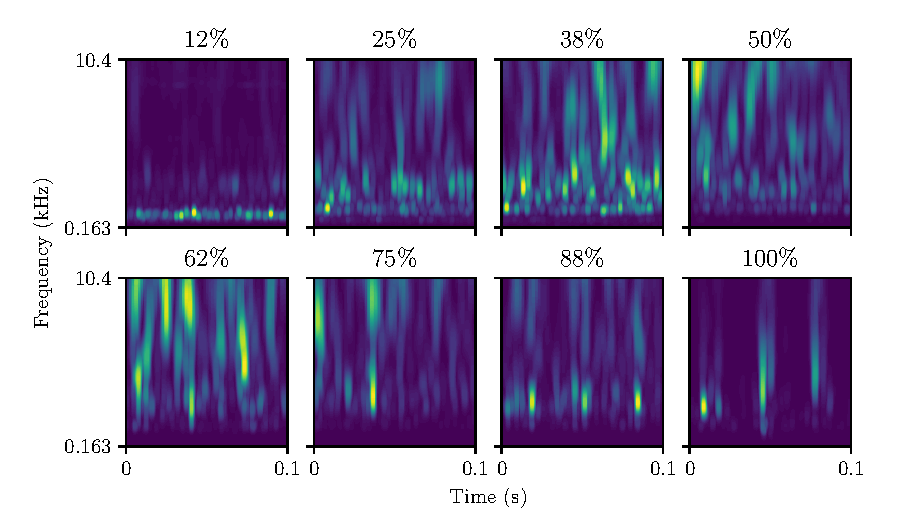
\includegraphics[]{figures/femtocwt_scaleograms_h.pdf}
	\caption{Scaleograms of different stages of Bearing1\_1 life (horizontal vibrations)}%
	\label{fig:bearings_fault_progress_scaleograms_h}
\end{figure}

\begin{figure}[h]
	\centering
	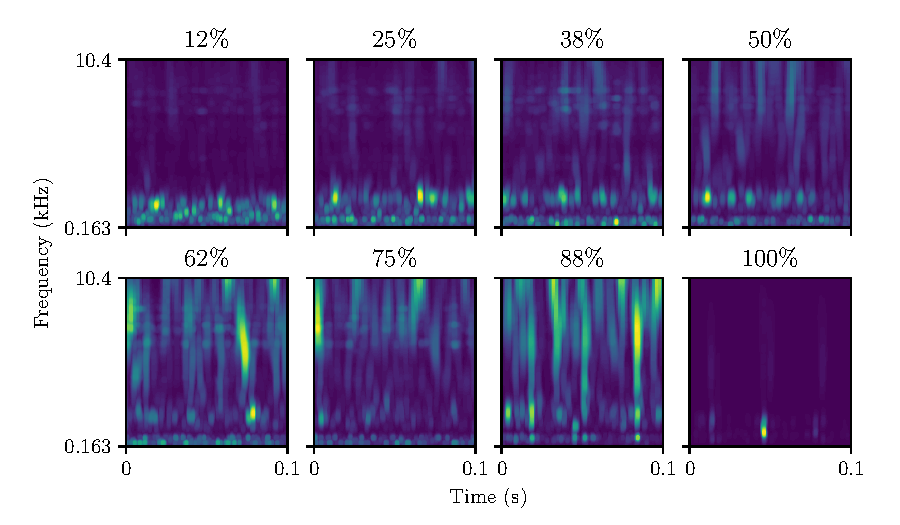
\includegraphics[]{figures/femtocwt_scaleograms_v.pdf}
	\caption{Scaleograms of different stages of Bearing1\_1 life (vertical vibrations)}%
	\label{fig:bearings_fault_progress_scaleograms_v}
\end{figure}

Scaleograms can show important information about the bearing's health state, but different bearings can have different degradation patterns. For this reason, a dataset of scaleograms extracted from vibration data is constructed. The first 80 vibration snapshots from each bearing are considered to represent a healthy bearing, while the last 80 vibration snapshots are considered faulty. This is considered as a binary classification task, where a convolutional neural network will be used to automatically extract features from scaleograms (both horizontal and vertical vibration data scaleograms) dataset and classify the bearing's health state. To avoid complexity and the cost of training a large model, the scaleograms are resized to a shape of (128$\times$128), so the input to the network is of shape (2$\times$128$\times$128) where the two channels correspond to both horizontal and vertical vibration scaleograms. This data represents bearings from the first operation condition (from Bearing1\_1 to Bearing1\_7).

\subsection{Detecting bearings failure using convolutional neural networks}%
\label{sub:detecting_bearings_failure_using_convolutional_neural_networks}

\subsubsection{Network architecture}%
\label{subsub:network_architecture}
For this task, a convolutional neural network (\acrshort{cnn}) with 3 convolutional layers, 3 maxpooling layers and 3 fully-connected layers is used. The complete network architecture with the number of parameters in the network is represented in Table \ref{table:scaleograms-classifier-architecture}.

\begin{table}[ht]
    \centering
    \begin{tabu}{lll}
\tabucline[1.5pt]{-}
\textbf{Layer (type)}   & \textbf{Output shape} &   \textbf{Param \#} \\
\tabucline[1pt]{-}
Conv1 (Conv2D)		&	(None, 2, 128, 16)	&	18448\\
MaxPool1 (MaxPooling2D) &    (None, 1, 64, 16)		&	0\\
Conv2 (Conv2D)          &    (None, 1, 64, 32)         	&	4640\\
MaxPool2 (MaxPooling2D) &    (None, 1, 32, 64)         	&	0\\
Conv3 (Conv2D)          &    (None, 1, 32, 128)        	&	18496\\
MaxPool3 (MaxPooling2D) &    (None, 1, 16, 128)        	&	0\\
Flatten1 (Flatten)      &   (None, 2048)              	&	0\\
Dense1 (Dense)          &    (None, 1024)              	&	524800\\
Dropout1 (Dropout)	&	(None, 512)		&	0\\
Dense2 (Dense)          &    (None, 64)                	&	32832\\
Dropout2 (Dropout)	&	(None, 64)		&	0\\
Dense3 (Dense)          &    (None, 2)                 	&	66\\
\tabucline[1pt]{-}
Total params: 559,346 &				&	\\
Trainable params: 599,346				&	\\
Non-trainable params: 0&				&	\\
	\tabucline[1.5pt]{-}
    \end{tabu}
    \caption{Bearings health state classifier architecture}
    \label{table:scaleograms-classifier-architecture}
\end{table}

\subsubsection{Training process}%
\label{subsub:training_process}
Generated dataset contained a total of 1120 samples, 716 samples were used for training, 180 for validation and 224 for test. The network was trained for 50 epochs with batch size of 64 samples. Figure \ref{fig:scaleogram-classifier-training} shows the training process.

\begin{figure}[H]
	\centering
	\includegraphics{figures/femtocwt_training.pdf}
	\caption{Bearings health state classifier training}%
	\label{fig:scaleogram-classifier-training}
\end{figure}

\subsubsection{Results discussion}%
\label{subsub:results-discussion}
The network achieved a perfect training accuracy of 100\% and similar validation and test accuracy of around 98\%. Table \ref{table:femto-cwt-results} shows loss and accuracy on train, validation and test data. Table \ref{table:femto-cwt-metrics} shows the additional precision, recall and F-1 score metrics.

\begin{table}[H]
	\centering
	\begin{tabu}{lcc}
		\tabucline[1.5pt]{2-3} 
		&			\textbf{Perte}	&	\textbf{Exactitude}	\\
	   \tabucline[1pt]{-}
		Ensemble d'entraînement &	0.0017	&	100.00\%		\\
		Ensemble de validation 	&	0.0528 	&	98.89\%			\\
		Ensemble de test	&	0.0527 	&	98.44\%			\\
   \tabucline[1.5pt]{-}
   \end{tabu}
   \caption{Résultats de l'entraînement}
   \label{table:femto-cwt-results}
\end{table}

\begin{table}[H]
	\centering
	\begin{tabu}{cc}
		\tabucline[1.5pt]{1-2} 
		\textbf{Metric} & \textbf{Value}	\\
	   \tabucline[1pt]{-}
		Precision	&	0.9896		\\
		Recall	 	&	0.9694		\\
		F1 Score	&	0.9794		\\
   \tabucline[1.5pt]{-}
   \end{tabu}
   \caption{Additional metrics for network performance}
   \label{table:femto-cwt-metrics}
\end{table}

Figure \ref{fig:bearings_health_state_classifier_roc} shows the ROC curve of the classifier:

\begin{figure}[H]
	\centering
	\includegraphics[]{figures/femtocwt_roc_auc.pdf}
	\caption{Bearings health state classifier ROC curve on test set}%
	\label{fig:bearings_health_state_classifier_roc}
\end{figure}

\subsection{The need for new prognostics features}%
\label{sub:the_need_for_appropriate_features}
The prognostic model's input is vital to its predictions accuracy \cite{coble2009} and since that's the case, a feature selection step should be carried out while developing the model, which aims to select a set of appropriate features that can make the prediction more accurate \cite{javed2012}. That's why it's important to use concrete metrics which can quantify the quality of our selected prognostics features and help comparing them directly and select the most suitable ones.

\subsubsection{Trendability and monotonicity}%
\label{subsub:trendability_and_monotonicity}
In \cite{coble2009} the authors proposed a set of metrics which can be used to quantify the quality of prognostics features and directly compare their suitability for use in predictive models, two of these metrics are \textbf{monotonicity} and \textbf{trendability}. According to their defiition, monotonicity refers to the nature of the variable whether it is increasing or decreasing and it has a value between 0 and 1 where a variable that is always increasing or decreasing will have monotonicity of 1. Monotonicity is defined by equation \ref{equation:monotonicity}: 
\begin{equation}
	M=\frac{\text{no. of }\frac{d}{dx} > 0}{n-1} - \frac{\text{no. of }\frac{d}{dx} < 0}{n-1}
\label{equation:monotonicity}
\end{equation}

Trendability on the other hand was defined as whether a given feature follows the same trend (increasing or decreasing) across a population of systems. A feature that is always decreasing or increasing have a higher trendability than another one that doesn't follow a specific trend across different cases. Accordingly, trendability is defined by equation \ref{equation:trendability}:  

\begin{equation}
	\begin{aligned}
		t_i&= \frac{\text{no. of }\frac{d}{dx}>0}{n-1}+\frac{\text{no of } \frac{d^2}{dx^2}>0}{n-2}\\
Trendability&=1-std(t_i)
	\end{aligned}
	\label{equation:trendability}
\end{equation}

\subsection{Trigonometric features and cumulative descriptors}%
\label{sub:trigonometric_features}
In \cite{javed2013} the authors proposed a new feature extraction procedure from vibration data based on discrete wavelet transform (Section \ref{subsub:discrete_wavelet_transform}) and trigonometric functions. Firts, the raw vibration signal is decomposed using discrete wavelet transform with db4 wavelet and 4th level of decomposition, then the decomposition coefficients are scaled using trigonometric functions (e.g. asinh, atan), finally standard deviation of the scaled coefficients is calculated to obtain the final value. According to the authors, these features are less sensitive to noise and variability of raw vibration signals. 

Table \ref{table:trigonometric-classic_features} shows mathematical definition of different classic and trigonometric features used in litearture:

\begin{table}[ht]
    \centering
    \begin{tabu}{ll}
		\tabucline[1.5pt]{-}
		\textbf{Trigonometric features}   & \textbf{Formula} \\
		\tabucline[1pt]{-}
		Standard deviation of asinh &   $\sigma\left(log\left[x_j+\sqrt(x_j^2+1)\right]\right)$  \\
		Standard deviation of atan  &   $\sigma\left(\frac{i}{2}log\left(\frac{i+x_j}{i-x_j}\right)\right)$ \\
					    &  \\
		\textbf{Classic features} & \textbf{Formula}\\
		\tabucline[1pt]{-}
		Entropy & $E(x)=\sum_jE(x_j)$ \\
		Energy & $e=\sum_{j=0}^nx_j^2$\\
		Root mean square & $RMS=\sqrt{\frac{1}{n}(x_1^2+\ldots+x_n^2)}$\\
		Skewness &  $\frac{\sum_{j=1}^n(x_j-\bar{X})^3}{(n-1)\sigma^3}$\\
		Kurtosis &  $\frac{\sum_{j=1}^n(x_j-\bar{X})^4}{(n-1)\sigma^4}$\\
		Upper bound & $max(x)+\frac{1}{2}\frac{max(X)-min(X)}{n-1}$\\
	\tabucline[1.5pt]{-}
    \end{tabu}
    \caption{Prognostics trignonometric and classic features \cite{javed2013}}
    \label{table:trigonometric-classic_features}
\end{table}

Figure \ref{fig:trigonometric_features_bearing1_1} shows two trigonometric features (asinh and atan) for Bearing1\_1 from FEMTO dataset. They have been filtered using Savitsky--Golay filter to reduce noise and variability.

\begin{figure}[h]
	\centering
	\includegraphics[width=0.8\linewidth]{figures/trigonometric_features.pdf}
	\caption{Trigonometric features of Bearing1\_1}%
	\label{fig:trigonometric_features_bearing1_1}
\end{figure}


Even that trigonometric features are less susceptible to noise compared to classical features (e.g. rms, skewness, kurtosis, etc.), that's not always the case. The authors also proposed the use of cumulative descriptors (i.e. running total) in order to assure monotonicity of the features. The cumulative feature associated with each feature is calculated according to equation \ref{equation:cumulative_features} :

\begin{equation}
Cf_{nk} = \frac{\sum_{i=1}^n f_{ik}} {\sqrt{abs\left(\sum_{i=1}^nf_{ik}\right)}}
\label{equation:cumulative_features}
\end{equation}

In Figure \ref{fig:trig_classic_cumulative_features} cumulative classic and trigonometric features are compared to their non-cumulative counterparts. Even with only visual inspection it is apparent that using cumulative descriptors greatly enhances the quality of prognostics features by reducing noise and fluctuations. 

\begin{figure}[H]
	\centering
	\includegraphics[width=0.8\linewidth]{figures/trig_classic_cumulative_features.pdf}
	\caption{Classic and trigonometric cumulative features}%
	\label{fig:trig_classic_cumulative_features}
\end{figure}

To quantify the enhancement caused by using cumulative descriptors on prognostics features, monotonicity and trendability for each feature and its cumulative counterpart is calculated and summarized in Tables \ref{table:trigonometric-classic-monotonicity} and \ref{table:trigonometric-classic-trendability} respectively.

\begin{table}[ht]
\centering
\begin{tabu}{cc|cc}
\tabucline[1.5pt]{-}
Feature & Monotonicity & Cumulative Feature & Monotonicity \\
\hline
$\sigma(atan)$ & 0.486 & C-$\sigma(atan)$ & 1 \\
$\sigma(asinh)$ & 0.481 & C-$\sigma(asinh)$ & 1 \\
kurtosis & 0.059 & C-kurtosis & 0.998 \\
entropy & 0.035 & C-entropy & 1 \\
rms & 0.481 & C-rms & 1 \\
ubound & 0.287 & C-ubound & 1\\
\tabucline[1.5pt]{-}
\end{tabu}
\caption{Monotonicity difference between trigonometric and classic features and their cumulative descriptors}
\label{table:trigonometric-classic-monotonicity}
\end{table}

\begin{table}[ht]
\centering
\begin{tabu}{cc|cc}
\tabucline[1.5pt]{-}
Feature & Trendability & Cumulative Feature & Trendability \\
\hline
$\sigma(atan)$ & 0.987 & C-$\sigma(atan)$ & 0.993 \\
$\sigma(asinh)$ & 0.989 & C-$\sigma(asinh)$ & 0.995 \\
kurtosis & 0.985 & C-kurtosis & 0.890 \\
entropy & 0.994 & C-entropy & 0.976 \\
rms & 0.988 & C-rms & 0.993 \\
ubound & 0.990 & C-ubound & 0.996\\
\tabucline[1.5pt]{-}
\end{tabu}
\caption{Trendability difference between trigonometric and classic features and their cumulative descriptors}
\label{table:trigonometric-classic-trendability}
\end{table}

It is very obvious that features monotonicity increased significantly for cumulative features compared to non-cumulative ones. But for trendability the difference was less significant. Figure \ref{fig:features_fitness} plots both monotonicity (x-axis) and trendability (y-axis) of both types of features:

\begin{figure}[H]
	\centering
	\includegraphics{figures/featuresfitness.pdf}
	\caption{Features fitness}%
	\label{fig:features_fitness}
\end{figure}

\section{Application to oilfield equipment}%
\label{sec:application_to_oilfield_equipment}

\subsection{Top Drive}%
\label{sub:top_drive}

In oil drilling rigs, Top Drive is a device that is used to turn the drillstring and replace the conventional rotary table and kelly. The main advantage of Top Drives over conventional solutions is the ability to drill using three joints of pipes instead of just one, thus reducing drastically drilling time. Top Drives also helps drillers to minimize the cost and frequency of stuck pipe incidents \cite{slbtopdrive}.

Figure \ref{fig:figures/bentec_500_ht} shows Bentec 500-HT Top Drive.

\begin{figure}[h]
	\centering
	\includegraphics[width=0.9\linewidth]{figures/bentec_500_ht.jpg}
	\caption{Topdrive Bentec 500-HT}%
	\label{fig:figures/bentec_500_ht}
\end{figure}

From an engineering perspective, Top Drives are much more complicated systems than conventional rotary table and kelly, thus they need more rigorous maintenance programs to ensure their availability considering their major role in drilling operations. Every year the oil and gas technology is pushed harder, to drill in harder conditions and to drill deeper and more challenging oil wells, this poses stricter requirements on used equipment: to be able under and sustain harsher conditions while maximizing its availibility which is of great importance in the field, for example  Top Drives downtime cost can reach 1m\$ per day and cause significant delay to drilling operations \cite{skfbrochure}. 

In \cite{Pournazari2016} the authors reported an industry survey that was conducted to assess the impression of different groups of people (operators, contractors, rig builders…) on the usage of Top Drives. The survey showed an average 60\% satisfaction level across all the groups in the survey, which is an indicative that Top Drives aren't really meeting the expectations in the industry. They were also asked which are the features they would like to see in Top Drives, the most wanted things are less downtime and better ability to detect failures before the breakdown of the system. This means that a more reliable preventive maintenance and prognostics approach is the most wanted improvement to these systems in the field.

\subsection{Top Drive components}%
\label{sub:top_drive_components}

Top Drives are made of many subassemblies which are shown in Figure \ref{fig:topdrive-subassemblies}\footnote{All the following figures of Top Drive components were taken from Bentec technical bulletin for TD-500-HT and TD-350-HT Top Drives}.

\begin{figure}[H]
	\centering
	\includegraphics[width=\linewidth]{figures/topdrive_subassemblies.png}
	\caption{Bentec 500-HT Top Drive subassemblies}%
	\label{fig:topdrive-subassemblies}
\end{figure}

The Top Drive subassembly of interest here is the drilling unit (Figure \ref{fig:topdrive-drillingunit}) which is responsible for generating the rotation motion and transfering it to the drillstring. Drilling unit is composed of protection frame, hydraulic unit, mudd supply, hanger assembly and\textemdash the most important for the current discussion\textemdash a drive.

\begin{figure}[H]
	\centering
	\includegraphics[width=.7\linewidth]{figures/topdrive_drillingunit.png}
	\caption{Bentec 500-HT Top Drive drilling unit}%
	\label{fig:topdrive-drillingunit}
\end{figure}

The drive itself is composed of:

\begin{itemize}
	\item Engine cooling system
	\item Brake
	\item AC Motor
	\item Gearbox (Figure \ref{fig:topdrive-drillingunit-drive-components}(a))
	\item Mainshaft (Figure \ref{fig:topdrive-drillingunit-drive-components}b)
\end{itemize}

\begin{figure}[H]
	\centering
	\begin{subfigure}[t]{0.4\textwidth}
         \centering
	 \includegraphics[width=.7\textwidth]{figures/topdrive_drillingunit_drive_gearbox.png}
	 \label{fig:topdrive-drillingunit-drive-gearbox}
	 \caption{Drive gearbox}
     \end{subfigure}%
     \begin{subfigure}[t]{0.4\textwidth}
         \centering
 \includegraphics[width=0.7\textwidth]{figures/topdrive_drillingunit_drive_mainshaft.png}
	 \label{fig:topdrive-drillingunit-drive-mainshaft}
	 \caption{Drive mainshaft}
     \end{subfigure}
	\caption{Main components of the drive}%
	\label{fig:topdrive-drillingunit-drive-components}
\end{figure}

The gearbox has two stages with transmission ratio of 14:1. The speed of the engine is reduced twice then transferred to the bullgear (1) of the gearbox. The bullgear is located on the thrust bearing. Lubrification of the gearbox is done with combined splash/pressure librification (3). The mainshaft (4) is powered by the bullgear of the gearbox and located in the gearbox with the thrust bearing (2) and it is conducted via lower bearing (3). A wash pipe (1) is connected to execute drilling fluid. The mainshaft also holds the load collar (5) which bears the link adapter to the drill pipe. 

Figure \ref{fig:skf_tapered_roller_thrust_bearing} shows an example of a tapered bearing usually used in Top Drives. While Figure \ref{fig:skf_topdrive} shows the bearing within a Top Drive.

\begin{figure}[H]
	\centering
	\includegraphics[width=0.6\linewidth]{figures/skf_tapered_roller_thrust_bearing.png}
	\caption{SKF tapered roller thrust bearing \cite{skf_tapered_roller_thurst_bearing}}%
	\label{fig:skf_tapered_roller_thrust_bearing}
\end{figure}

\begin{figure}[H]
	\centering
	\includegraphics[width=0.7\linewidth]{figures/skf_topdrive.png}
	\caption{Bearing position within the Top Drive \cite{skf_bearing}}%
	\label{fig:skf_topdrive}
\end{figure}

\subsection{Proposed approach for Top Drive monitoring using neural networks}%
\label{sub:proposed_approach_for_top_drive_monitoring_using_neural_networks}

Top Drives are already equipped with many sensors to monitor their state like temperature, pressure and flow sensors, yet information that these sensors is only used in a simplified manner by operators \cite{Pournazari2016}. In order to improve maintenance programs and adopt preventive maintenance and prognostics approaches, a more sophisticated and methodological approach to process data provided by these sensors need to be employed, along with introduction of new vibration sensors which are the main monitoring sensors used for bearings and gears, the elements which are present in the top drive and are work under high and varying loads.

Figure \ref{fig:topdrive-drive-sensors} is a simplified schematic representation of the proposed procedures to employ additional sensors (red dots) for vibrations in the drive to monitor different elements like gears and bearings. Enough sensors should be installed to capture vibrations in the three axes: vertical, horizontal and axial vibrations. When the Top Drive is in use, data collected from these sensors can be used to develop a neural network architecture to detect bearings degradation (Section \ref{sec:case_study_bearings_faults_prognostics_using_neural_networks}) or---if enough historic data is available---classifying different degradation patterns (Section \ref{sec:case_study_bearings_faults_diagnostics_using_neural_networks}). Correctly detecting degradation or even classifying degradation patterns can be used to plan and prepare the appropriate maintenance actions and execute them in the appropriate time before any serious degradation happens which may cause serious non-productive time and high corrective maintenance costs. 

\begin{figure}[H]
	\centering
	\begin{tikzpicture}
	\tikzstyle{gear} = [rectangle,  draw, align=center, darkgray, fill=gray, text=white]
	\tikzstyle{bearing} = [rectangle, draw, align=center]
	\tikzstyle{shaft} = [rectangle, draw, minimum width = 1em, fill=darkgray, darkgray]
	\tikzstyle{sensor}  = [circle, fill,red, minimum size=5,inner sep=0]
	\draw[black!20!white, thick, fill=black!5!white ] (0,0) rectangle (18em,-8em);
	\node[] at (2.5em,-1em) {Gearbox};

	\node[gear, minimum width=8em, minimum height=2em] at (7em,-4em) (gear) {Gear};
	\node[gear, minimum width=4em, minimum height=2em, right = 0em  of gear] (pinion) {Pinion};

	\node[bearing, minimum width=7em, minimum height=2em, below = 0em of gear] (thrustbearing) {\footnotesize Thrust bearing};

	\node[shaft, minimum height=4em, above = 0em of pinion] (shaft) {};
	\node[draw, thick, minimum width=3em, rounded corners, radius=3,minimum height=5em, above = 0em of shaft] {AC Motor};

	\node[shaft, minimum height=3em, below = 0em of thrustbearing] {};

	\node[sensor, below = 0em of thrustbearing] {};
	\node[sensor, left = 0em of thrustbearing] {};
	\node[sensor, above = 0em of gear] {};
	\node[sensor, left = 0em of gear] {};
	
\end{tikzpicture}	

	\caption{Proposed additional vibration sensors to monitor the drive}%
	\label{fig:topdrive-drive-sensors}
\end{figure}

\section{Conclusion}
This chapter adopted a data generation approach from literature that converts vibration signals into images. Vibration signals used here corresponds to bearings with different types of faults and fault diameters. After converting raw signals into images, a \acrshort{cnn} is used to classify transformed signals (i.e. images) into their corresponding faults types and diameters. The model achieves near-perfect classification accuracy on the test set.
